% !Mode:: "TeX:UTF-8"
% !TEX program  = xelatex

%\documentclass{cumcmthesis}
\documentclass[withoutpreface,bwprint]{cumcmthesis} %去掉封面与编号页
\usepackage[framemethod=TikZ]{mdframed}
\usepackage{url}   % 网页链接
\usepackage{subcaption} % 子标题
\usepackage{enumitem}
\usepackage{geometry}
\usepackage{booktabs}

\geometry{left=2.5cm,right=2.5cm,top=2.5cm,bottom=2.5cm}
\title{“同心协力”策略研究}
\tihao{B}
\baominghao{201901001015}
\schoolname{北京大学}
\membera{刘宇林}
\memberb{蒋衍}
\memberc{董婉萍}
\supervisor{}
\yearinput{2019}
\monthinput{09}
\dayinput{15}
\begin{document}

 \maketitle
 \begin{abstract}
本文根据题目的要求,对“同心协力”游戏项目的过程进行深入分析,结合实际情况,考虑了可能出现的不同条件、影响因素,在合理的抽象及假设之下,建立数学模型,确定除了游戏最优策略,从而达到连续颠球的次数尽可能多的目的。

首先从理想状态出发,假设队员的发力可以精确控制,经过对过程的受力分析及计算,我们只需要让队员提供恒力,使得每次发力后,排球获得的的能量与碰撞过程中损失的能量相等,从而排球弹跳过程稳定为周期运动,即可达到目标。

再考虑现实情形中,队员发力时机和力度不可能做到精确控制,存在一定误差,于是鼓面可能出现倾斜。通过计算,我们确定了队员的发力时机和力度与某一特定时刻的鼓面倾斜角度的关系,并制定出了相应的调整策略。对于具体的出现误差的实例,我们又相应地给出了具体的调整策略,并进一步分析在现实情形中这种调整策略的实施效果。

最后我们分析了模型的误差来源,从准确性、稳定性、适用性角度,对模型进行了评估和改进,并对模型的推广方向进行了展望,具有一定参考意义。

\keywords{刚体力学\quad  动量\quad   受力分析\quad  最优策略}
\end{abstract}

%目录  2019 明确不要目录,我觉得这个规定太好了
%\tableofcontents

%\newpage

\renewcommand\thesection{\arabic{section}}
\section{问题重述}
“同心协力”是一项团队协作能力拓展项目。该项目的道具是一面牛皮双面鼓,鼓身中间固定多根绳子,绳子在鼓身上的固定点沿圆周呈均匀分布,每根绳子长度相同。团队成员每人牵拉一根绳子,使鼓面保持水平。项目开始时,球从鼓面中心上方竖直落下,队员同心协力将球颠起,使其有节奏地在鼓面上跳动。颠球过程中,队员只能抓握绳子的末端,不能接触鼓或绳子的其他位置。

项目所用排球的质量为270g。鼓面直径为40cm,鼓身高度为22cm,鼓的质量为3.6kg。队员人数不少于8人,队员之间的最小距离不得小于60cm。项目开始时,球从鼓面中心上方40cm处竖直落下,球被颠起的高度应离开鼓面40cm以上,如果低于40cm,则项目停止。项目的目标是使得连续颠球的次数尽可能多。

我们的任务是,根据题目给出的不同条件,建立数学模型解决以下问题:
\begin{enumerate}
\item 在理想状态下,每个人都可以精确控制用力方向、时机和力度,试讨论这种情形下团队的最佳协作策略,并给出该策略下的颠球高度。
\item 在现实情形中,队员发力时机和力度不可能做到精确控制,存在一定误差,于是鼓面可能出现倾斜,建立模型描述队员的发力时机和力度与某一特定时刻的鼓面倾斜角度的关系。
\item 在现实情形中,根据问题2的模型,是否需要调整问题1中给出的最优策略?如果需要,如何调整?
\item 当鼓面发生倾斜时,球跳动方向不再竖直,于是需要队员调整拉绳策略。假设人数为10,绳长为2m,球的反弹高度为 60cm,相对于竖直方向产生1°的倾斜角度,且倾斜方向在水平面的投影指向某两位队员之间,与这两位队员的夹角之比为1:2。为了将球调整为竖直状态弹跳,请给出在可精确控制条件下所有队员的发力时机及力度,并分析在现实情形中这种调整策略的实施效果。
\end{enumerate}

\section{问题分析}
图\ref{fig:mol}给出了题述情境的几何示意图,上方球体为排球,下方圆柱体为同心鼓,四周发出的射线为各队员手中控制的绳子。当队员们松开绳子时,同心鼓获得向下的速度,位置向下移动,同时绳端向中心移动,绳子与竖直方向的夹角变小;用力拉紧绳子时,同心鼓获得向上的速度,位置向上移动,同时绳端向外侧移动,绳子与竖直方向的夹角变大。初始排球从空中自由下落,与鼓面碰撞时弹起,获得向上的速度,同心鼓在力的作用下,向下运动,后回到碰撞原点,与下落的排球发生再次碰撞,形成往返运动。游戏的目标即使排球弹起方向尽量平稳,并且每次弹起高度都超过40cm。

\begin{figure}
	\centering
	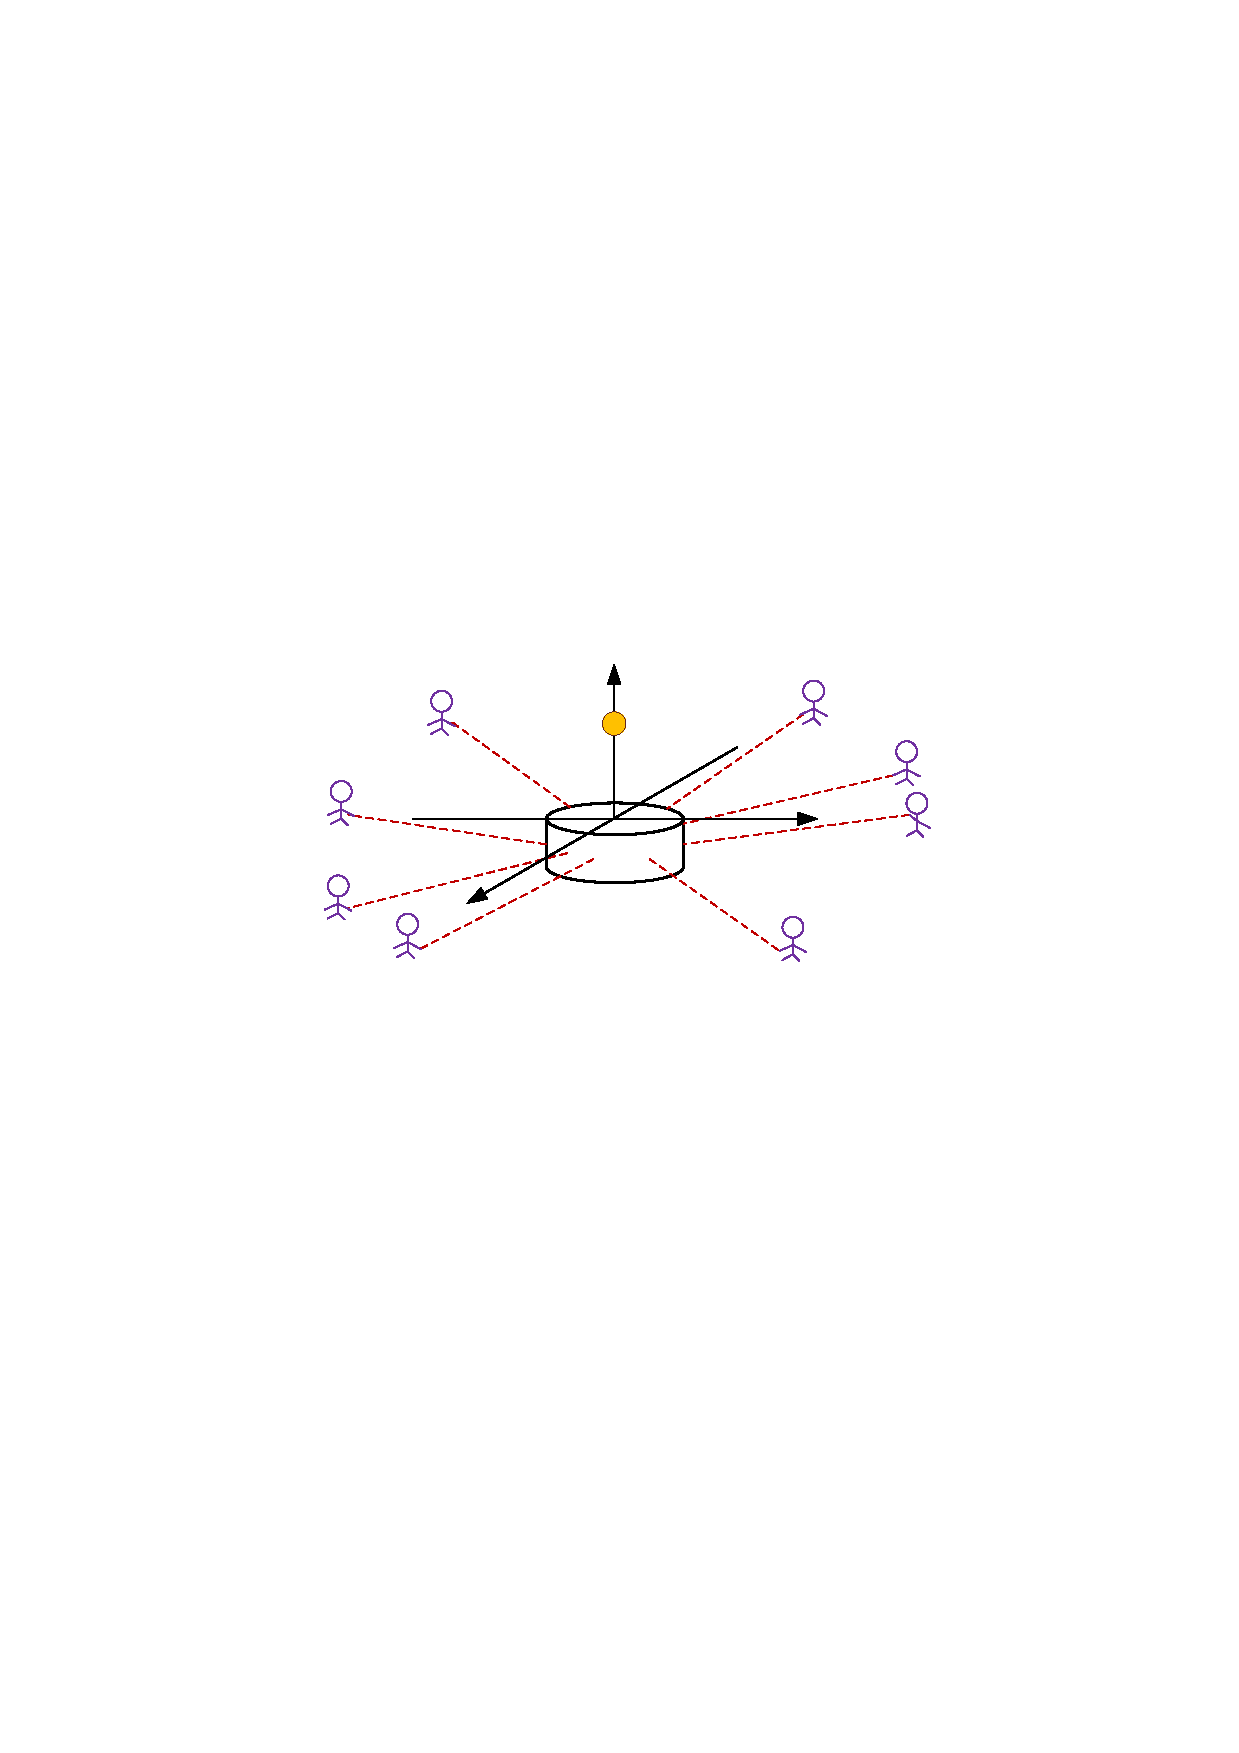
\includegraphics[width=.6\textwidth]{mol.pdf}
	\caption{几何示意图}
	\label{fig:mol} %此处的label相当于一个图片的专属标志,目的是方便上下文的引用
\end{figure}

此系统的理想状态是排球和鼓都恰在竖直方向作周期运动,每次弹起高度相同,如若每名队员都能精确控制用力方向、时机与力度,不难找到一组使系统保持平稳周期运动的参数。但现实中难以做到精确控制,从而会发生弹起高度不足或球轨迹歪斜掉出鼓面,导致游戏失败。

本文旨在制定出现实条件下,“同心协力”游戏的团队最佳协作策略。其中第一部分从理想状态出发,得到精确控制下,团队的最佳协作策略,并给出该策略下的颠球高度;第二部分,我们计算了发力时机和力度与某一特定时刻的鼓面倾斜角度的关系;第三部分,我们根据第二部分中的数据,分析现实情况中的随机因素对理想模型的干扰,进一步对策略进行调整,从而得到现实条件下的最佳策略;第四部分,我们以具体实例为背景,探究了排球跳动方向倾斜后的调整策略,并分析了调整策略的实施效果。

\section{符号约定}
由于运动复杂,涉及数据众多,因此我们将要用到大量符号。在此部分只列出部分重要的符号,其它符号在出现的部分会说明含义。
\begin{longtable}[c]{cc}
    \caption{符号使用与说明}\label{tab:001}\\
        \toprule[1.5pt] 符号 & 含义\\ \hline \hline \endfirsthead %1第一页表头
        \toprule[1.5pt]  符号 & 含义\\ \hline  \hline \endhead %2续页表头
        $M$ & 鼓的质量\\
        \hline
        $m$ & 排球的质量\\
        \hline
        $r$ & 鼓的半径\\
        \hline
        $l$ & 绳子的长度\\
        \hline
        $h$ & 鼓质心的高度\\
        \hline
        ${F}$ & 人拉绳子的力\\
        \hline
        $T$ & 排球弹起落下一个周期的时长\\
        \hline
        $v_1$ & 鼓在与球碰撞前的速度\\
        \hline
        $v_1^{'}$ & 鼓在与球碰撞后的速度\\
        \hline
        $v_2$ & 球在与鼓碰撞前的速度\\
        \hline
        $v_2^{'}$ & 球在与鼓碰撞后的速度\\
        \hline
        $\overrightarrow{L}$ & 鼓的角动量\\
        \hline
        $\theta$ & 绳与竖直方向的夹角\\
        \hline
        $\overrightarrow{\omega}$ & 鼓的角速度\\
        \hline
        $I$ & 鼓的转动惯量\\
        \bottomrule[1.5pt]
\end{longtable}

\section{模型假设}

\begin{enumerate}
	\item 绳子的劲度系数极大,不考虑其长度变化;
	\item 所有人握绳端处的高度相同;
	\item 鼓和排球都可视为刚体,自身不发生形变;
	\item 不考虑风与空气阻力的一切影响;
	\item 不考虑排球自身的旋转;
	\item 排球与鼓面碰撞时不在鼓面滑动;
	\item 所有碰撞都符合牛顿碰撞定律,且都在瞬间完成。
\end{enumerate}

\section{模型建立与求解}
以鼓质心所在竖直线上与手握处平齐为原点,以过鼓质心且与鼓面平行的任一直线及其水平面上的垂线为x,y轴、竖直方向为z轴,建立空间直角坐标系如图\ref{fig:mol}。

\subsection{精确控制下的运动模型}
初始时排球从40cm高度静止落下,排球与鼓各自在z轴方向作周期运动。为消除不确定因素,使排球与鼓保持平稳的周期运动,在此设定二者运动周期相同,排球每次弹起高度都为40cm,每个周期球与鼓碰撞一次,碰撞点为$(0,0,0)$。
\subsubsection{排球的运动模型}
在我们设定的条件下,排球每次弹起达到相同高度,故需每次与鼓面碰撞后都有相同的初速度,且与碰撞前速度等大反向,撞后仅受重力作用,故有方程\ref{eq:velo}
\begin{equation}
\left\{
\begin{array}{lr}
v_2^{'}=-v_2 \\
\frac{1}{2}g(\frac{T}{2})^2=0.4m
\end{array}
\right.
\label{eq:velo}
\end{equation}
其中$v_1, v_2, v_1^{'}, v_2^{'}$均取沿z轴向上为正,向下为负。所有符号代表的值均为国际制单位。
\subsubsection{鼓的运动模型}
在不与排球碰撞时,鼓仅受到各队员拉力与自身重力的作用。由于队员均匀站在周围,x、y轴方向上的受力相互抵消,因此仅z轴方向的合力非零,
鼓在z轴方向受力状况如\ref{eq:drumF}
\begin{equation}
Ma=nF\cos\theta-Mg
\label{eq:drumF}
\end{equation}
\subsubsection{球鼓碰撞}
假设球鼓碰撞服从牛顿碰撞定律,法向相对速度在碰撞前与碰撞后比值恒定,满足方程\ref{eq:newton}
\begin{equation}
	e=\frac{|v_2^{'}-v_1^{'}|}{|v_2-v_1|}
	\label{eq:newton}
\end{equation} 
其中$e$为碰撞系数,只与碰撞物体材质有关而与碰撞速度无关。查阅资料估计球与鼓面的碰撞系数$e=0.9$。
值得注意的是,由于鼓自身的高度,球鼓碰撞点并不与鼓的质心相重合。
\subsubsection{模型求解}
由排球弹起最高点为40cm不难解出运动周期与排球和鼓的撞前、撞后速度如\ref{eq:velo}
\begin{equation}
\left\{
\begin{array}{lr}
T = 0.5714 \\
v_2 = -2.8,\ v_2^{'} = 2.8 \\
v_1 = 0.3684,\ v_1^{'} = -0.0514
\end{array}
\right.
\label{eq:velo}
\end{equation}
\begin{figure}
	\centering
	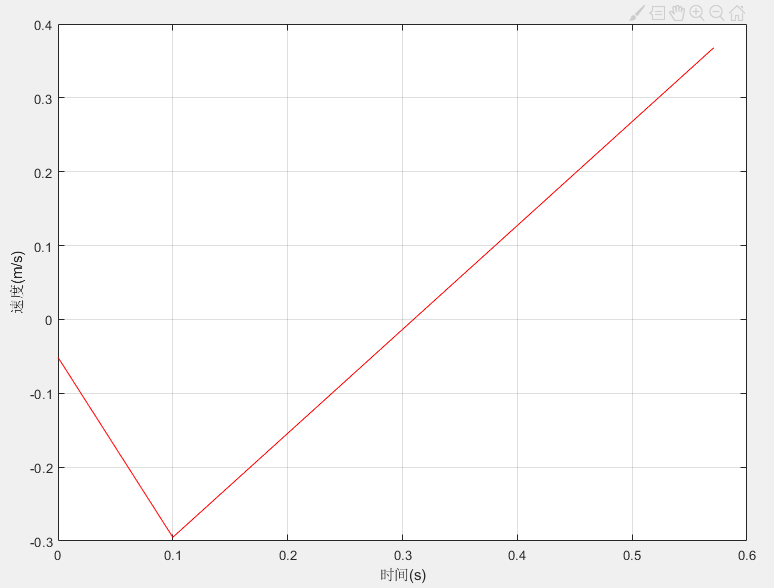
\includegraphics[width=.6\textwidth]{v.png}
	\caption{一个周期内的v-t图}
	\label{fig:vt} %此处的label相当于一个图片的专属标志,目的是方便上下文的引用
\end{figure}
因此队员们需要控制用力时机与大小,使得鼓在一个周期T内走过的位移和量恰好为零,碰撞前后速度恰符合上述要求。
为简化用力策略,不妨将周期T分为两阶段,每阶段鼓以不同的加速度做匀加速运动。设鼓在周期内第一段时间$t_1$以恒定加速度$a_1$运动,
在周期内第二段时间$t_2$以恒定加速度$a_2$运动,$v-t$图如图\ref{fig:vt}所示。周期内运动参数满足方程\ref{eq:eq}.
\begin{equation}
\left\{
\begin{array}{lr}
\frac{1}{2}(2v_1^{'}+a_1t_1)t_1 + \frac{-(v_1^{'}+a_1t_1)^2}{2a_2}+\frac{v_1^2}{2a_2} = 0 \\
v_1-(v_1^{'}+a_1t_1) = a_2t_2 \\
t_1 + t_2 = T
\end{array}
\label{eq:eq}
\right.
\end{equation}
方程\ref{eq:eq}中未知量有$t_1, t_2, a_1, a_2$,不妨取$t_1=0.1$,即解得$a_1 = -2.4354,\ a_2 = 1.4071$.
根据第一阶段与第二阶段不同的运动状态,有第一阶段的$h$与$F$解析式如方程\ref{stage1},第二阶段解析式如方程\ref{stage2}

\begin{equation}
\left\{
\begin{array}{lr}
h=h_0+v_1^{'}t+\frac{1}{2}a_1t^2\\
F=\frac{ML}{nh}(g+a_1)
\end{array}
\right.
\label{stage1}
\end{equation}

\begin{equation}
\left\{
\begin{array}{lr}
h=h_1+v^{'}(t-t_1)+\frac{1}{2}a_2(t-t_1)^2\\
F=\frac{ML}{nh}(g+a_2)
\end{array}
\right.
\label{stage2}
\end{equation}
取人数为8即$n=8$,代入数据解得$F$最终解析式为\ref{eq:sol}, 一个周期内每位队员发力$F$与时间$t$的函数图像如图\ref{fig:Ft}
\begin{equation}
F=
\begin{cases}
\frac{6.6281}{-0.11+0.5t^2-0.0514t}& \text{t<0.1}\\
\frac{10.0864}{-0.0908+0.7036t^2-0.4356t}& \text{0.1<t<0.5714}
\end{cases}
\label{eq:sol}
\end{equation}

\begin{figure}
	\centering
	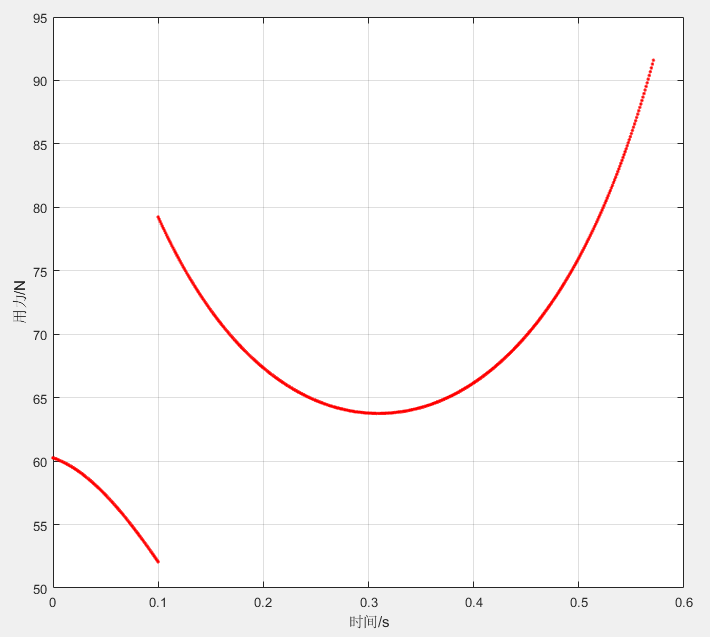
\includegraphics[width=.6\textwidth]{Ft.png}
	\caption{一个周期内的F-t图}
	\label{fig:Ft} %此处的label相当于一个图片的专属标志,目的是方便上下文的引用
\end{figure}

\subsection{操作误差下的鼓面倾斜模型}
队员在实际操作中难免出现发力时机与力度偏离策略规划的情况。本部分旨在建模分析发力时机与力度的误差对鼓倾斜角度的影响。
鼓自身为刚体,由题目条件,受到八个队员的拉力与重力共9个力。由于考虑鼓面倾斜角度时不需考虑排球的影响与鼓的平动,因此我们只考察鼓在各队员拉力作用下的转动。

\subsubsection{计算转动惯量}
易知鼓在不均匀拉力下转动的转轴平行x-y平面。转动惯量计算式为$I=\sum mr^2$,在此例中用微元法计算鼓的转动惯量。
由于鼓为中空,故在此将鼓视为由若干个矩形框组合而成,对每个矩形框的四条边分别求转动惯量小量后再积分,得到鼓的转动惯量:
$$I=\int_{0}^{0.4} \frac{m_{1}l_{1}^{2}+3m_{1}l_{2}^{2}+m_{2}l_{2}^{2}+3m_{2} l_{1}^{2}}{6(2\pi r^{2}+ 2\pi rh)}dz=0.02536$$
其中$m_1$,$m_2$分别是矩形框的长$l_1$宽$l_2$的质量

\subsubsection{转动过程分析}
根据题述发力时机与力度的取值,我们将所有误差组合分为两类:
\begin{itemize}
	\item 如果所有人同时发力而力度有所差异时,根据每人的力度计算鼓所受力矩,设力的大小与方向在$\Delta t$时间内不变,
	鼓面倾角为鼓在做匀加速转动$\Delta t$时间后转过的角度
	\item 如果有人提前发力,则将鼓的转动分为两段$\Delta t$时间,第一段时间前所有人的力度(姑且称“基准力”)恰能使鼓静止在题述初始位置,
	第一段时间开始时提前发力者增大力度而其他人保持基准力,第二段时间所有人开始发力,鼓在两段时间内分别做匀加速转动	
\end{itemize}
\begin{figure}[h]
	\centering
	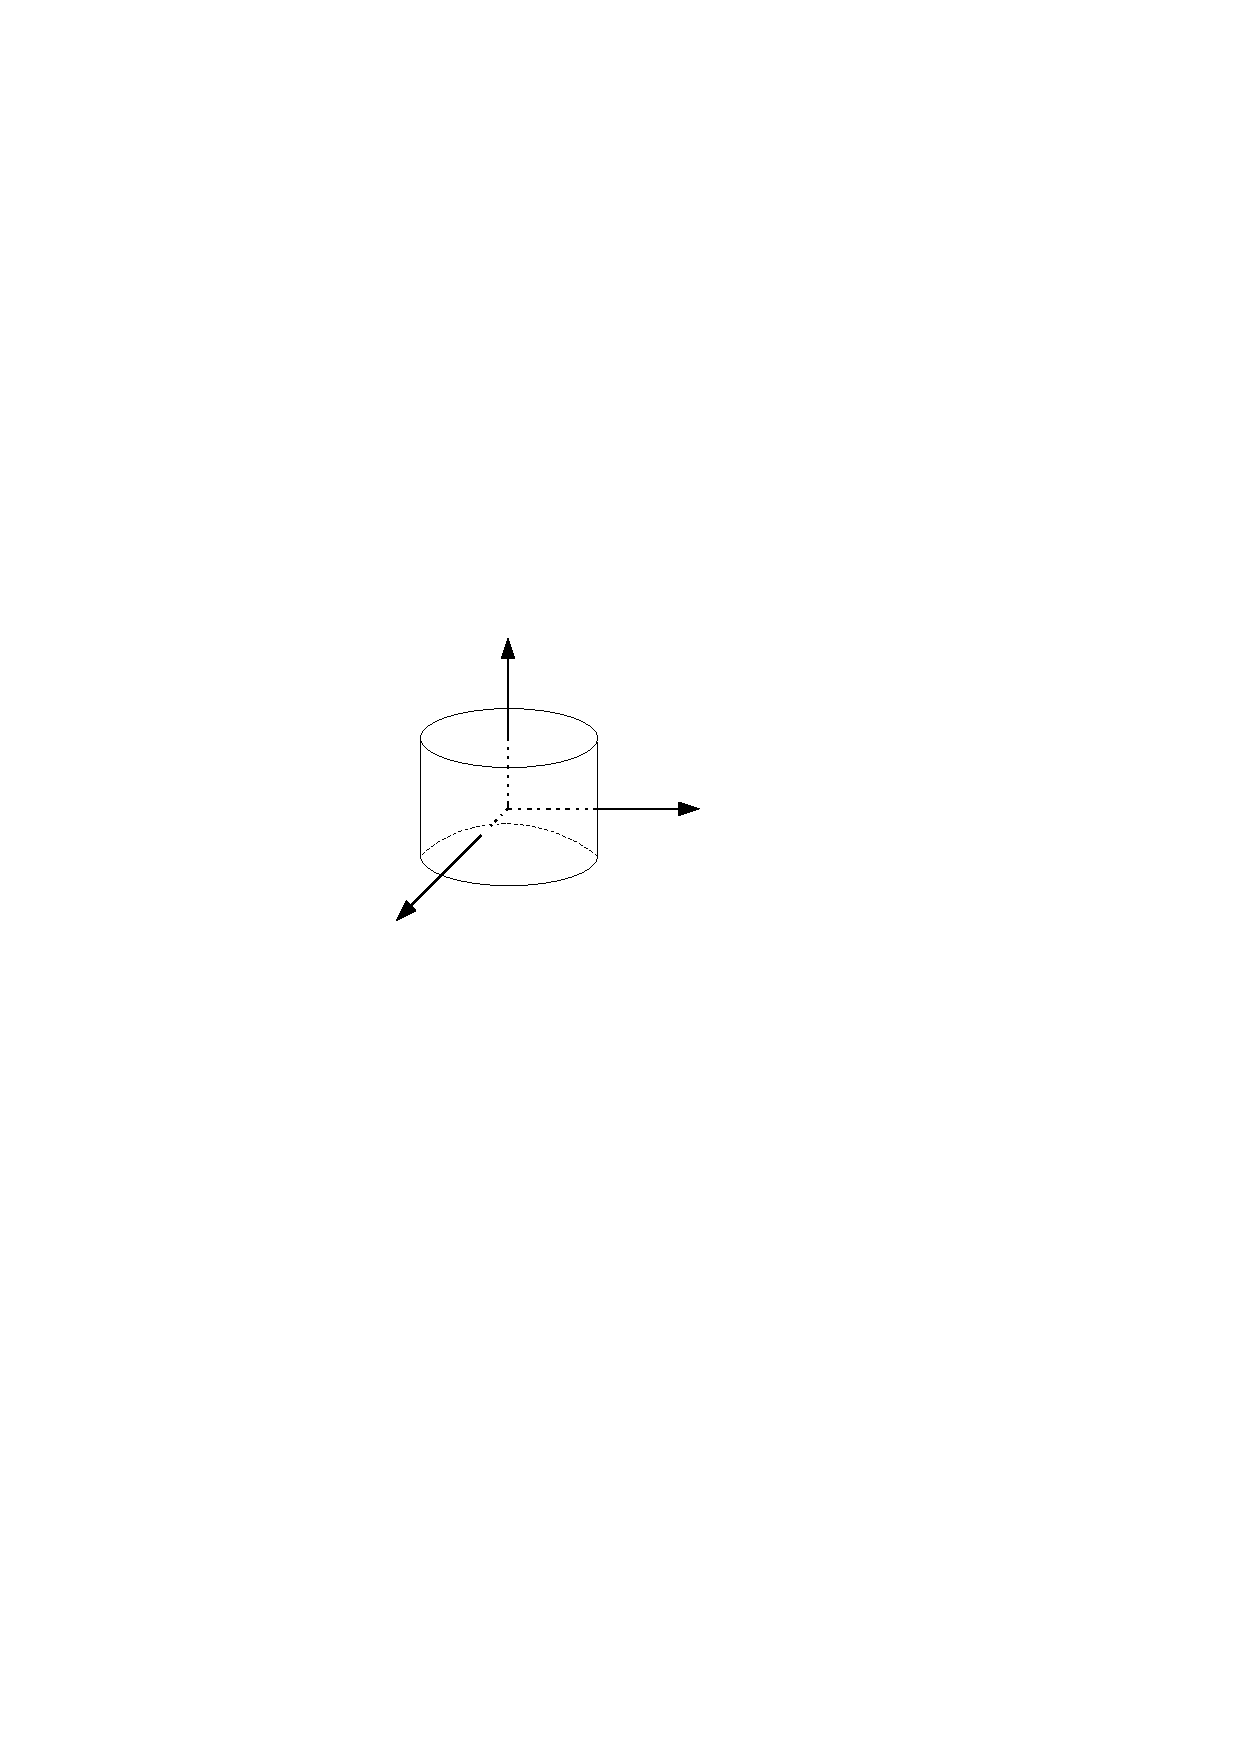
\includegraphics[width=.6\textwidth]{col.pdf}
	\caption{鼓面倾斜分析}
	\label{fig:col} %此处的label相当于一个图片的专属标志,目的是方便上下文的引用
\end{figure}
根据题述条件,在此取$\Delta t=0.1$. 已鼓的质心为原点,水平方向两垂直直线为x、y轴,竖直方向为z轴建立空间直角坐标系如图\ref{fig:col}.
八位队员等间距地站在鼓四周,绳子间两两夹角为45°如图\ref{fig:per},拉力方向斜向上。

\begin{figure}[h]
	\centering
	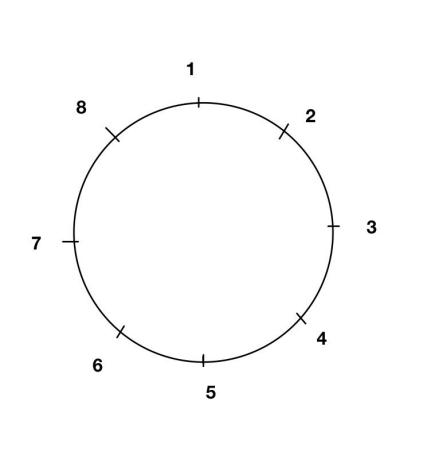
\includegraphics[width=.6\textwidth]{person.png}
	\caption{8名队员的位置与编号}
	\label{fig:per}
\end{figure}

对于误差组合类型1,鼓面倾斜计算步骤如下:
\begin{itemize}
	\item 计算出8人各自拉力向量$\overrightarrow{F_1},\overrightarrow{F_2},...,\overrightarrow{F_8}$,在此重力对鼓旋转无贡献,故不考虑;
	\item 由$\overrightarrow{L}=\sum \overrightarrow{r}\times \overrightarrow{F}\Delta t$得到出鼓在$\Delta t$内获得的角动量;
	\item 由$\omega=\frac{\overrightarrow{L}}{I}$得到$\Delta t$后的最终角速度
	\item 由$\Delta \phi=\frac{1}{2}\omega \Delta t$得到匀加速转动转过的角度
\end{itemize}
对于误差组合类型2,同样经上述步骤1~2得到出第一阶段结束时的角动量$\overrightarrow{L_1}$,再带入第二阶段每位队员的力度得到第二阶段的角动量增量$\overrightarrow{L_2}$,再带入总角动量$\overrightarrow{L}=\overrightarrow{L_1}+\overrightarrow{L_2}$到步骤3~4求得第二阶段末的角速度. 将两阶段转过的角度矢量合成即得到最终角度。计算所用matlab源代码见附件。

\subsubsection{题述情形求解}
见表\ref{cli}

\begin{table}[h]
	\centering
\begin{tabular}{|c|c|c|c|}% 通过添加 | 来表示是否需要绘制竖线
	\hline  % 在表格最上方绘制横线
	序号 & 鼓面倾角(°) & 序号 & 鼓面倾角(°)\\
	\hline  % 在表格最上方绘制横线
	1 & 1.4619 & 6 & 1.3254 \\
	\hline  %在第一行和第二行之间绘制横线
	2 & 2.7013 & 7 & 11.0462 \\
	\hline  % 在表格最上方绘制横线
	3 & 1.1189 & 8 & 4.1790 \\
	\hline  %在第一行和第二行之间绘制横线
	4 & 1.7317 & 9 & 8.6602\\
	\hline  % 在表格最上方绘制横线
	5 & 3.1998 & & \\
	\hline % 在表格最下方绘制横线
\end{tabular}
\caption{题述情形求解}
\label{cli}
\end{table}

\subsection{随机误差下的调整模型}
在第一问中我们我们给出了在可以精确控制用力以及用力时机的策略并给出了力与时间的关系,但是实际上把握用力大小和时机是非常困难的,在第二问中我们分别用理论分析和计算机计算算出了在给定情况下鼓的倾角,在第三问中我们将结合一二问的模型,引入影响力和时间的随机向量($f_dis,t_dis$),对击鼓过程中出现的情况进行全面考量,并给出相应的调整策略。
\subsubsection{补充假设}
\begin{enumerate}
\item 第一问给出了理想状态下力和时间的关系,如图\ref{fig:Ft},在此假设出现“特殊情况”(即发力时机和力度出现误差)仅有可能存在于力发生突变的位置。

这与事实是相符的,在持续发力时,不易出现失误,而在调整力的瞬间,由于人体无法精确感知力的大小与时间,很容易导致偏差,所以我们假设只在第0.1s时和一个周期结束时($t=\frac{4}{7}$),才会出现第二问中发力时机和力度的扰动。而在一个周期结束前(即球还没撞到鼓时),力不会提前变化,故可能出现误差的时间为$0s$之后以及$0.1s$左右的一小段(以第一周期为例)。在本模型中,我们仅探究在$t=0.1s$左右的扰动。
\item 扰动值近似为正态分布,即($f_{dis},t_{dis}$)$\~{}$($f_{base}*N(0,1),t_{base}*N(0,1)$)

根据问题2数据,我们取base值为(10,0.1),得到在$t=0.1s$左右的数据,用计算机模拟出i组数据,$t_{i,j}$表示第i组数据中第j人的扰动,f类似,可以得到如下表格(F(t)为上图所示的力与时间的函数)。特别规定若$\mid t_{i,j}\mid>0.05$则剔除。(i亦可理解为第i周期)
\begin{figure}[h]
	\centering
	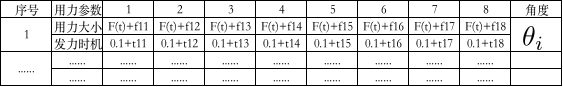
\includegraphics[width=.6\textwidth]{table.png}
	\caption{随机误差下的角度关系}
	\label{fig:table}
\end{figure}

\item 扰动一直持续到0.15s,也即在这之后,所有力恢复为$F(t)$。

结合问题2的数据以及我们的计算,在0.05s时鼓已经发生肉眼可见的角度变化,考虑到队员在发现扰动后会进行调整,我们取扰动时间为0.05s,也即出现误差的时间段为$(0.1+t_{i,j})s\~{}0.15s$,之后为调整时间。这也隐含了我们的又一假设,即人的反映时间为0s,在发现出现倾斜后可以迅速做出调整,且精确控制调整用力。
\end{enumerate}

\subsubsection{倾角计算}
根据扰动开始时间($0.1+t_{i,j}$)从小到大进行排序,设第y个人最先发生扰动(允许多人同时发生扰动,这里仅设一个),此时他用力$F(0.1+t_{i,j})+f_{i,y}$,其余人用力为$F(0.1+t_{i,j})$,用问题2中第一问的方法,计算出下一人出现扰动时刻的倾角$\theta_{i1}$以及此时的角速度。随后,第z个人发生扰动,用问题2最后一问的方法,计算出倾角为$\theta _{i2}$(注意角速度的合成),同理直到时间到达0.15s,此时倾角为$\theta_{i}$,角速度为$\omega_i$。

\subsubsection{实际过程模拟及策略}
\begin{enumerate}
\item 排球的跳动高度不能过高,弹起方向与鼓面法线的角度不能大于10°。以鼓面直径40cm计算,若鼓面不移动且排球弹起点为鼓面圆心,则当排球的弹起角度出现10°时倾斜时,当球的跳动高度为56.7cm时,球会落出鼓面。而要尽量使得球的跳动保持竖直状态,球与鼓面的接触点以落在距鼓面圆心20cm的范围内为最佳。这样算来,球在鼓面的跳动高度以60cm以内为好。
\item 尽量不要靠鼓面击打排球,只需要让球在水平的鼓面借助鼓面的弹性和排球的弹性自然跳动即可,只有当发现球的高度过低时才进行发力。这样可以减少发力次数,有利于发力效果更加稳定,并且使排球跳动高度不会过高。
\item 队员相互配合,尽量控制发力时间与发力大小一致。
\item 使得排球与鼓面接触位置稳定在距鼓面圆心20cm的范围内,当接触点偏离时,队员共同发力,调整位置,使接触点回归圆心。
\item 尽量保持鼓面水平,当鼓面出现倾斜使得排球偏移时,作出适当调整。
\end{enumerate}

\subsection{鼓面倾斜校正模型}
\subsubsection{模型概述}


\section{模型的模拟与检验}

对于问题一中精确控制的模型,我们用微元法,从初始状态出发,以$\Delta t=0.001$为步进求出鼓与排球每个时刻的位置、速度与受力情况,
检验排球是否能被周期性地弹起至要求高度。我们用matlab编程模拟了上述过程,源代码见附件2.

5s内的运动模拟结果如图\ref{fig:moni}所示,图\ref{fig:moni}左红线与蓝线分别为排球与鼓的高度随时间变化的曲线,
右为排球速度随时间变化的曲线。此处排球与鼓都沿z轴方向位移,遂取z轴向上方向为正。从图上可看出排球与鼓做同步的周期运动,右图速度图像是图\ref{vt}在t正半轴上的完美周期性延拓。由于浮点误差排球弹起高度并非每次都达到40cm,但即使不足时也与40cm的高度要求相差不到2cm,很好的说明了模型结果的正确性。

\begin{figure}[h]
	\centering
	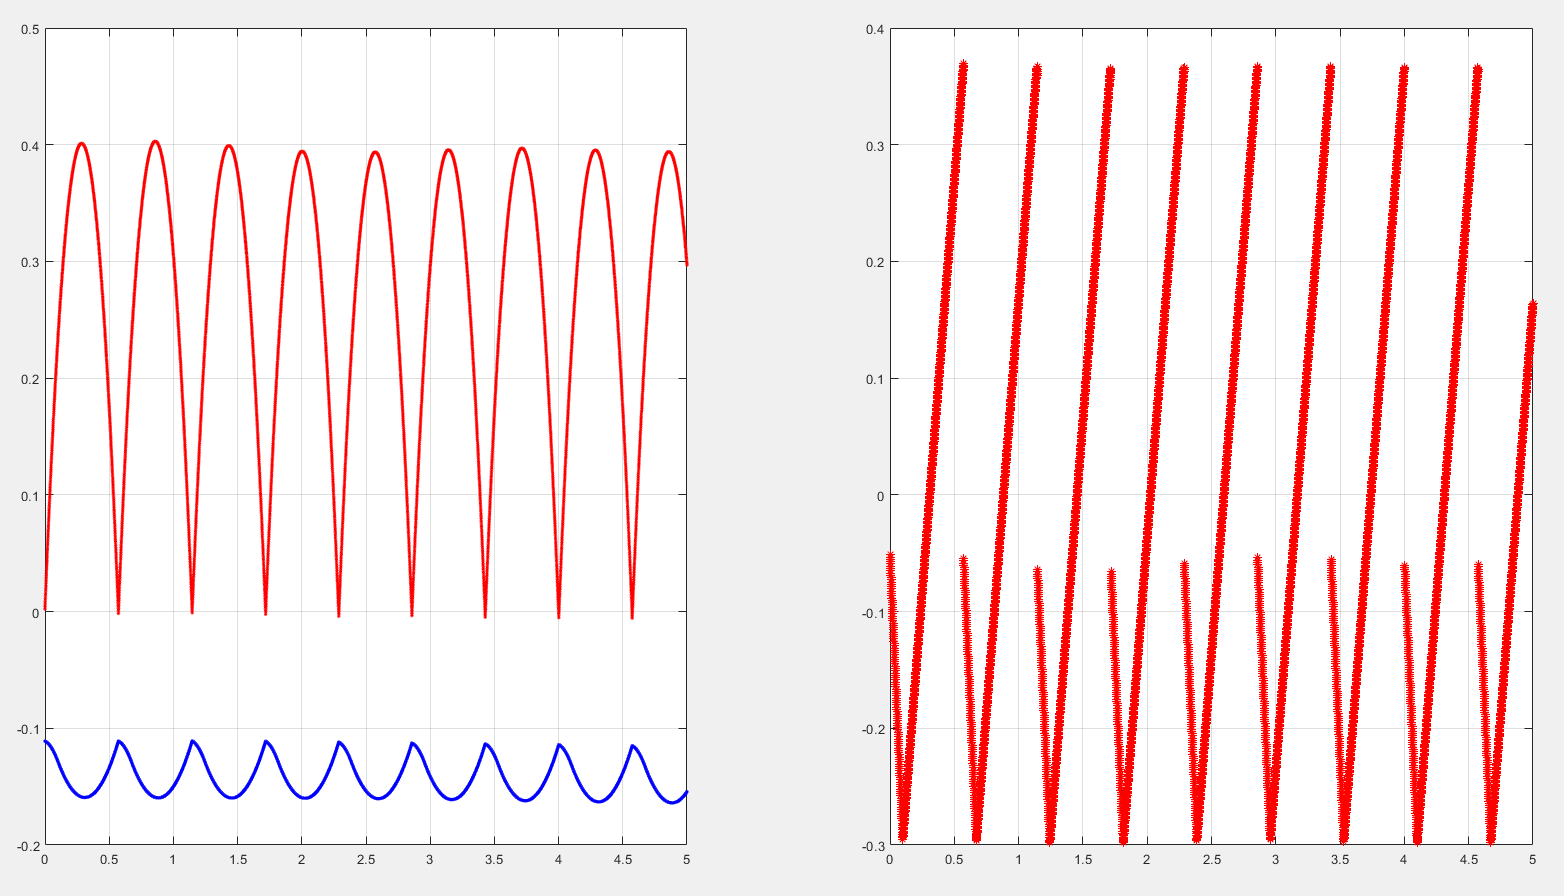
\includegraphics[width=.9\textwidth]{moni.png}
	\caption{精确控制模拟}
	\label{fig:moni}
\end{figure}

\section{误差分析}

\subsection{空气阻力}
空气阻力是物体下落过程中影响速度的重要因素。查阅资料得物体在介质运动所受的空气阻力满足式\ref{eq:ff}
\begin{equation}
	f=\frac{1}{2}c\rho Sv^n
	\label{eq:ff}
\end{equation}
其中$c$为空气阻力系数,与介质性质与物体形状有关,$\rho$是介质密度,$S$是物体垂直于运动方向的截面面积。在低速运动即$v<10m/s$情形下取$n=1$. 因此得排球下落最快时($v=2.8m/s$)所受空气阻力$f=0.0827N$,仅为所受重力的约$3\%$,因此我们认为忽略空气阻力并不会造成可观的误差。

\subsection{鼓面静摩擦力}
实际情况中排球与鼓面都粗糙,倾斜碰撞的瞬间鼓与之间存在相对滑动趋势,加之排球碰撞时可能处于旋转状态,会导致排球接触鼓面的短时间内受到沿鼓面方向的摩擦力。

假设已知排球与鼓面间摩擦系数$\mu$,将碰撞前排球速度$v_2$分解为垂直于鼓面的分量$v_\bot$与平行于鼓面的分量$v_\parallel$;碰撞后的速度分解为$v'_\bot$和$v'_\parallel$。由牛顿碰撞定律球与鼓面碰撞后,两物体在垂直鼓面方向的相对速度变为原来的e倍。

为了证实这一点,我们对排球进行受力分析(如图)。垂直于鼓面的力$N$是由于排球形变产生的弹力,摩擦力为$f$,$N$与$f$夹角为$\gamma$。

排球与鼓面碰撞后的形变看作是弹性形变,碰撞后排球恢复了自己的形状,因而排球的弹性势能,在碰撞后重新变为排球的动能。换句话说,碰撞前后,排球沿鼓面法线方向运动的动能未变。而在摩擦力作用下,速度的平行分量发生了变化,摩擦力的方向与原平行分量的方向相反。如果排球与鼓面壁碰撞时不旋转,那么碰撞后的速度水平分量比$v_\parallel$小。这就是说,反射角$\beta$小于入射角$\alpha$,图1和图2所示的正是这样。如果碰撞前排球如图4所示方向旋转,当排球旋转得足够快时($\omega R>v_\parallel$),排球速度的水平分量向左,摩擦力的方向向右,并且速度的水平分量大于$v_\parallel$,这种情况下,反射角大于入射角。

另一种情况,当排球碰撞前不旋转,我们也认为,速度的水平分量不为零,在碰撞的过程中滑动并没有停止。弹力$N$是在球与鼓面接触时产生的,之后弹力$N$将逐渐增大,在排球形变达到最大程度时$N$达到最大值,此后$N$减小到零。在排球与鼓面碰撞过程中摩檫力$f$也不是常量,在任何时刻摩檫力的数学表达式为:
\begin{equation*}
	F_\textrm{摩}=\mu N
\end{equation*}
因此,在整个碰撞过程中,鼓面作用于球的合力的大小要改变,而方向不变。合力$Q$与鼓面法线的夹角为$\gamma$。由图3看出,$tan\gamma=\mu$,这样就有可能求出反射角。

根据牛顿第二定律,排球与鼓面碰撞时排球动量的变化量$\vartriangle P$与力$Q$同时产生。借肋于图2我们作出动量的变化量$\vartriangle P=m(v'-v)$(见图5)。
这个矢量与图3中的矢量$Q$一样,这个矢量与鼓面法线夹角为$\gamma$。由图5看出,
\begin{equation*}
	v'_\parallel=v_\parallel-2v_\bot tan\gamma
\end{equation*}
等式两端同除以$v_\bot$,并考虑到$\frac{v_\parallel}{v_\bot}=tan\alpha$,$\frac{v'_\parallel}{v'_\bot}=tan\beta$,$tan\gamma=\mu$,我们得到
\begin{equation*}
	tan\beta=tan\alpha-2\mu
\end{equation*}
一般而言,若排球碰撞前不旋转,则摩擦力会导致反射角小于入射角,由此可见摩擦力对模型精确程度确实有一定的影响。
\section{模型的优点与不足}
\subsection{模型的优点}
实际情况中,干扰因素可能有很多,条件也更复杂,我们对条件做了合理的假设与化简,适当舍去计算中的小量,从而使得计算难度相对降低,而模型拟合程度也较高。

在过程分析中,我们发现队员的发力点、所处的位置等条件,都会随机地发生一定的扰动,为了简化条件控制难度,我们将复杂的变量转化为用统一的物理量即发力的大小、角度等进行控制与表示,减少了模型所需的变量个数,从而降低了模型建立的难度与复杂程度。

在建立模型的过程中,通过视频资料,充分了解现实情况中,发力误差出现的来源。探究调整策略时,构造发力效果满足正态分布的随机数据,模拟现实情况中,队员发力时机和力度存在的误差,使得调整策略具有更稳定、更优良的实施效果。
\subsection{模型的不足}
短时间内空气阻力的影响可以忽略不计,但随着时间的延长,空气阻力的干扰程度逐渐增大,因此在建立长期模型时,还应将空气阻力纳入影响因素中。
\newpage

%参考文献
\begin{thebibliography}{9}%宽度9
    \bibitem[1]{mec}舒幼生. 力学(物理类). 2005.
    \bibitem[2]{nengliang} 葛松华, 王成金. 碰撞的能量转化和能量损失[J]. 青岛大学学报:自然科学版, 2000(3):40-42.
    \bibitem[3]{zuli}王立华. 空气阻力对自由落体运动的影响[J]. 沧州师范专科学校学报, 2000(2):50-52.
\end{thebibliography}


\newpage
\textbf{{\Large 附件一}}

计算问题二的matlab源代码

\begin{lstlisting}
	% 计算问题二
	i=0; h=0.11; l=1.7; L=0;  % h是初始质心高度, l是绳长, L是角动量
	I=0.0253595;   % 转动惯量
	t=acosd(h/l);  % 绳方向与竖直线夹角
	A=zeros(8,3); r=zeros(8,3); Fs=zeros(1,3);
	% A(i)是i号力向量,r(i)是i号发力点位移向量
	f90 = [1 4]; % 【修改】90N力的编号
	f80 = [];    % 【修改】80N力的编号
	% L =[0.0108, -0.0045, 0];  % 【修改】继承上一阶段角动量,在误差类型2中用到
	for deg = 0:45:359
	i = i+1;
	if ismember(i, f90) 
	F = 90;
	elseif ismember(i, f80)
	F = 80;
	else        % 【修改】正常发力大小,第一阶段是68.1545,第二阶段是80
	F = 80;
	end
	A(i,:) = [F*sind(t)*cosd(deg), F*sind(t)*sind(deg), F*cosd(t)];
	r(i,:) = [0.2*cosd(deg), 0.2*sind(deg), 0];
	L = L + cross(A(i,:), r(i,:))*0.1;  % 每个力矩都对角动量L有贡献,累加起来
	Fs = Fs + A(i,:);
	end
	w = L/I     % 角速度向量
	w_abs = norm(L)/I   % 角速度模长
\end{lstlisting}

\newpage
\textbf{{\Large 附件二}}

模拟问题一模型的matlab源代码

\begin{lstlisting}
	g = 9.8; n = 8; L = 2; e = 0.9; a1 = 2.4354; a2 = 1.4071;
	dt = 0.001; dxf = 0.0005; dx = dxf;tt = 0;
	drum = ball(3.6, -0.11, -0.0514, 0);
	vb = ball(0.27, 0, 2.8, -0.27*g);
	close;
	for t = 0:dt:4
	if (vb.h - drum.h < 0.11 && vb.v < 0 && drum.v > 0) 
	% 需要反弹
	v1p = drum.v; v2p = vb.v;
	M = drum.m; m = vb.m;
	drum.v = (M*v1p + m*v2p - e*m*(v1p-v2p))/(M+m);
	vb.v = e*(v1p-v2p) + drum.v;
	%v1p, drum.v
	end
	h1 = vb.h; h2 = drum.h;
	vb.h = vb.h + dt * vb.v;
	drum.h = drum.h + dt * drum.v;
	dx = max(abs(h1 - vb.h), abs(h2 - drum.h));
	dx = max(dx, dxf);
	
	vb.v = vb.v + dt * vb.F/vb.m;
	drum.v = drum.v + dt * drum.F/drum.m;
	
	tt = mod(t, 4/7);
	if tt < 0.1
	F_norm = -(drum.m*L/(n*drum.h)) * (g - a1);
	else
	F_norm = -(drum.m*L/(n*drum.h)) * (g + a2);
	end
	F = 0;
	for i=1:n
	F = F + normrnd(F_norm, 10);
	end
	drum.F = -g*drum.m - F*drum.h/L;
	
	subplot(1,2,1);
	plot(t, drum.h, 'b.');grid on; hold on
	plot(t, vb.h, 'g.');grid on; hold on
	subplot(1,2,2);plot(t, drum.v, 'r*');grid on; hold on
	end

\end{lstlisting}

\end{document} 